\documentclass{prologArticle}
\usepackage{float}
\usepackage{enumitem}
\usepackage{tabularx}
\usetikzlibrary{babel} % used to make edge possible


% use \declare{test/} to create a new variable nam\space
% you can use the root namespace too if you want to
% use \setvalue and \getvalue to manipulate data
\setvalue{meta/title =miniprojet - WhalEscape}
% Uncomment the line below to disable small caps in the section titles
\setvalue{formatting/section = \large\raggedright}

% If you want to use your own lststyle:
%\setvalue{formatting/listings/default = yourlststyle}

% \lstset{language=Java}
\newcolumntype{b}{X}
\newcolumntype{s}{>{\hsize=.3\hsize}X}
\newcolumntype{d}{>{\hsize=.8\hsize}X}

\begin{document}

\buildtitle



\section{Introduction}
Le but de ce projet était d'appliquer en pratique ce qui a été vu en cours durant le semestre. Pour cela il a fallu penser au dévelopement en prenant compte tout ce qui a été vu. Le temps imparti ne nous permettait pas de dévelloper tout les éléments d'un jeu-vidéo au maximum. Toutefois nous nous sommes efforcés de ne négliger aucun aspect général du jeu.

\section{Story}

\begin{figure}[H]
    \centering
    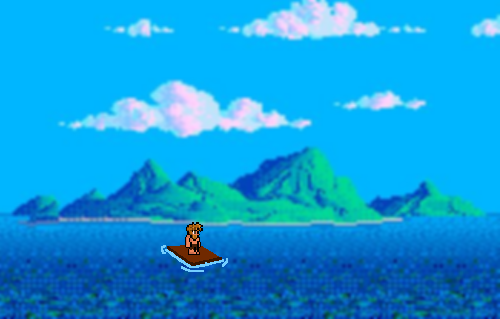
\includegraphics[width=0.6\textwidth]{res/story1.png}
    \caption{Jonah sur son radeau}
\end{figure}

\begin{figure}[H]
    \centering
    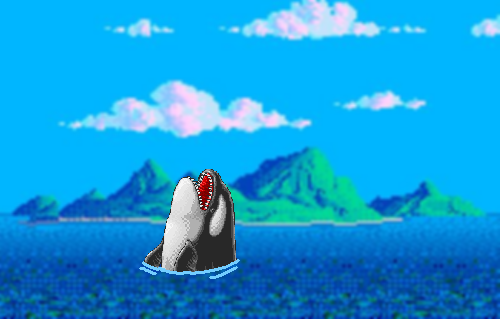
\includegraphics[width=0.6\textwidth]{res/story2.png}
    \caption{La baleine mange Jonah et son embarquation}
\end{figure}

Jonah a été victime d'un naufrage sur une île déserte. Seul survivant, il parvient a fabriquer un radeau et à quitter l'île. En s'éloignant de l'île, une baleine l'a attaqué et l'a avaler avec une partie de son radeau. Le joueur doit maintenant contrôller Jonah et l'aider à s'échapper de la baleine, en commençant dans les intestins. Il pourra utiliser les objets qu'il trouvera. Ces objets proviennent des restes du radeau ou ont été avalé par la baleine auparavant. Il devra aussi faire face à des ennemis tel que des blobs de sucs gastriques ou les restes d'autres naufragés malchanceux. Il devra remonter le système digestif de l'animal en passant par les intestincs et l'estomac avant d'atteindre l'évent qui lui permettera de sortir.

\begin{figure}[H]
    \centering
    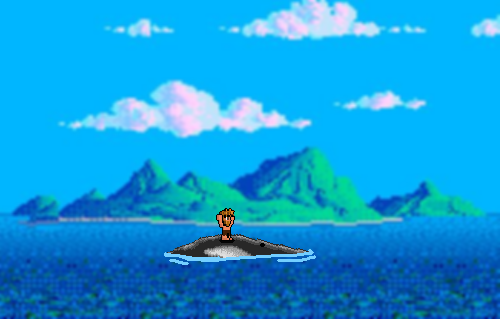
\includegraphics[width=0.6\textwidth]{res/story3.png}
    \caption{Jonah a réussi à sortir de la baleine}
\end{figure}

\section{Mechanics}

\subsection{Rules}

\subsubsection{Générales}
\begin{itemize}
    \item Si Jonah tombe dans le vide il meurt
    \item Jonah a X points de vie % TODO: A corriger
    \item À chaque fois qu'il se fait taper par un enemi, il perd un point de vie
    \item Lorsque Jonah n'a plus de points de vie il meurt
    \item Jonah peut attaquer seulement si il est équipé d'une rame
    \item Pour s'équiper de rame, il doit marcher dessus
    \item Au bout de 3 coups porté avec la rame, celle-ci échappe des mains de Jonah et il doit la ramasser à nouveau
    \item Lorsque Jonah meurt, il recommence au début du niveau
\end{itemize}

\subsubsection{Level 1}
\begin{itemize}
    \item Jonah doit trouver la zone qui le fera sortir de ce niveau
    \item Les enemis sont des squelettes d'autres naufragés malchanceux.
\end{itemize}

\begin{figure}[H]
    \centering
    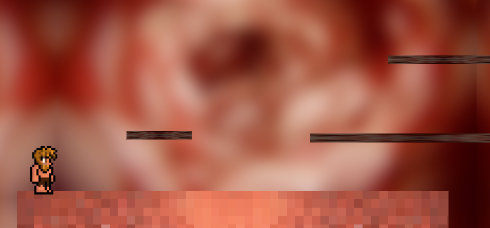
\includegraphics[width=0.8\textwidth]{res/level1.png}
    \caption{Départ du niveau 1}
\end{figure}

\subsubsection{Level 2}

\begin{itemize}
    \item Jonah doit monter les plateformes pour éviter de se faire ronger par l'acide gastrique qui remonte
    \item Si Jonah se fait toucher par l'acide (rattrapé par la caméra) il meurt
    \item Des blobs d'acides vont traverser l'écran afin de gêner Jonah dans sa progression
\end{itemize}

\begin{figure}[H]
    \centering
    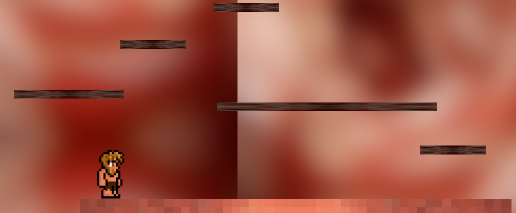
\includegraphics[width=0.8\textwidth]{res/level2.png}
    \caption{Départ du niveau 2}
\end{figure}

\subsection{Protagonist}

Le joueur se met dans la peau de Jonah un naufragé qui s'est fait gober par une baleine.

Verbes d'actions:
\begin{enumerate}
    \item déplacement gauche droite
    \item sauter
    \item attaquer si équipé d'une rame
\end{enumerate}

\subsection{Antagonists}

\subsubsection{Blob}
Une bactérie flottante se baladant tel un poisson rouge.

Verbes d'actions:
\begin{enumerate}
    \item Déplacement sinuosoidale gauche droite dans l'air
\end{enumerate}

\subsubsection{Squelette}
Les squelette d'anciennes victimes de la baleine veillent à ce qu'aucun intrus se balade dans le corps de la baleine. Ils patrouillent dans les intestins.

Verbes d'actions:
\begin{enumerate}
    \item Patrouille à pied de gauche à droite
    \item Attaquer si un ennemi se trouve devant lui.
\end{enumerate}

\subsubsection{Baleine}
Elle vous a gobé mais elle ne vas pas s'arrêter là, son corps est un véritable labyrinthe et plein de pieges.

Aucun verbe d'actions

\subsection{Minor}

\subsubsection{Carpe magique}
Déesse des pêcheurs, celle-ci vous veut votre bien et vous donnera de bons conseils pour vous en sortir.

Aucun verbe d'action




\section{Aesthetics}

\subsection{Aspect visuel}
Nous avons décidé de ne pas tout avoir en pixel art comme nous avions prévu au début. En effet nous étions pas capable de tout décider nous-mêmes. Pour beaucoup d'élément nous avons simplement pixelisé des photos existantes.

L'idée était de donner au maximum au joueur l'impression d'être dans un corps vivant sans trop le dégouter. Il a fallu flouter les photos d'estomacs que nous avions pour ne pas heurter la sensibilité de certain.

\subsubsection{Jonah}
Pour Jonah nous nous sommes fortement inspiré de l'image de Robinson Crusoé que les gens ont en tête.

\begin{figure}[H]
    \centering
    
\includegraphics[width=\textwidth]{res/jona_sheet.png}
    \caption{Les frames de déplacement de Jonah}
\end{figure}

\subsubsection{Blob}
L'idée avec le blobb était de faire quelque chose de semblable à l'idée que l'on peut se faire d'une molécule tout en restant simple pour pouvoir le dessiner facilement. La couleur verte a été choisie pour bien mettre en valeur que c'est un élément avec lequel on interagit dans le jeu.

\begin{figure}[H]
    \centering
    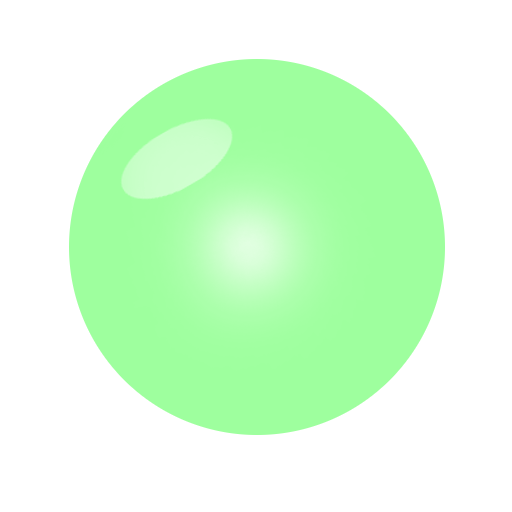
\includegraphics[width=0.1\textwidth]{res/blobb.png}
    \caption{L'illustration utilisé pour notre blobb}
\end{figure}

\subsubsection{Anticorp}
TODO à compléter avec l'image du squelette

\subsection{Aspect sonore}
Nous avons voulu donner le maximum de retour à l'utilisateur que nous pouvions. C'est pour cela que nous avions mis un son pour beaucoup d'élément. Tout nos éléments à part le thème du jeu sont issues du site internet "freesound"

\subsubsection{Jonah}
\begin{enumerate}
    \item Son lorsqu'il saute
    \item Son lorsqu'il frappe avec la rame
    \item Son lorsqu'il se fait toucher
\end{enumerate}

\subsubsection{Blobb}
Le blobb est plus a considéré comme une plateforme en mouvement qu'un personnage en termes d'actions. C'est pour ça que nous n'avons pas jugé approprié de lui mettre un son.

\subsubsection{Anticorp}
\begin{enumerate}
    \item Son lorsqu'il frappe
    \item Son lorsqu'il se fait toucher
\end{enumerate}


\subsubsection{Thème}
Pour la musique de thème nous avons utilisé un remix 8bit de la chanson thème de Pirates of the Carribean que l'on a trouvé libre de droits sur youtube.


\section{Technology}
Tout le jeu est fait avec Unity3D, avec C\# comme language de programmation.


\section{Conclusion}
Nous avons pris beaucoup de plaisir à faire ce projet. Nous avons pu explorer plus en détail des mécaniques d'Unity et explorer la multi-disciplanirité qu'est le dévellopement de jeu-vidéo. M

\end{document}
